% Scaled Dot-Product Attention — TikZ diagram
% Include in a LaTeX document with:
%   \usepackage{tikz}
%   \usetikzlibrary{shapes.geometric,arrows.meta,positioning}

\usetikzlibrary{shapes.geometric, arrows.meta, positioning}

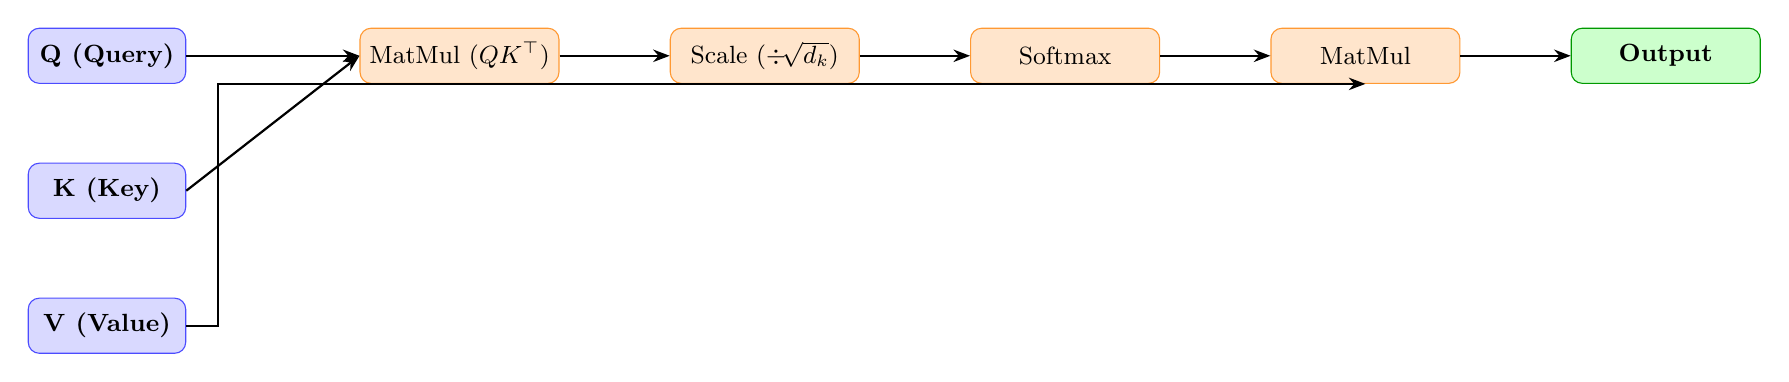
\begin{tikzpicture}[
  % Node styles
  inputnode/.style={
    rectangle, rounded corners=4pt,
    draw=blue!70, fill=blue!15,
    minimum width=2.0cm, minimum height=0.7cm,
    font=\bfseries\small
  },
  opnode/.style={
    rectangle, rounded corners=4pt,
    draw=orange!80, fill=orange!20,
    minimum width=2.4cm, minimum height=0.7cm,
    font=\small
  },
  outnode/.style={
    rectangle, rounded corners=4pt,
    draw=green!60!black, fill=green!20,
    minimum width=2.4cm, minimum height=0.7cm,
    font=\bfseries\small
  },
  % Arrow style
  arr/.style={-{Stealth[length=6pt]}, thick},
  node distance=1.0cm and 1.4cm
]

%% ── Input nodes ──────────────────────────────────────────────
\node[inputnode]                        (Q)      {$\mathbf{Q}$ (Query)};
\node[inputnode, below=of Q]            (K)      {$\mathbf{K}$ (Key)};
\node[inputnode, below=of K]            (V)      {$\mathbf{V}$ (Value)};

%% ── Operation column ─────────────────────────────────────────
\node[opnode,  right=2.2cm of Q]        (matmul1){MatMul ($QK^{\top}$)};
\node[opnode,  right=of matmul1]        (scale)  {Scale ($\div\!\sqrt{d_k}$)};
\node[opnode,  right=of scale]          (softmax){Softmax};
\node[opnode,  right=of softmax]        (matmul2){MatMul};

%% ── Output node ──────────────────────────────────────────────
\node[outnode, right=of matmul2]        (output) {Output};

%% ── Arrows: Q, K → MatMul1 ───────────────────────────────────
\draw[arr] (Q.east)  -- ++(0.4,0)  |- (matmul1.west);
\draw[arr] (K.east)  --             (matmul1.west);

%% ── Arrows: MatMul1 → Scale → Softmax → MatMul2 ─────────────
\draw[arr] (matmul1) -- (scale);
\draw[arr] (scale)   -- (softmax);
\draw[arr] (softmax) -- (matmul2);

%% ── Arrow: V → MatMul2 (entering from below) ─────────────────
\draw[arr] (V.east) -- ++(0.4,0) |- (matmul2.south);

%% ── Arrow: MatMul2 → Output ──────────────────────────────────
\draw[arr] (matmul2) -- (output);

\end{tikzpicture}
